\section{Resultados y análisis}
\begin{table}[!h]
	\centering
	\caption{Potencia medida en función de la distancia, a una temperatura fija.}
	\begin{tabular}{|c|c|}
		\hline
		Distancias(cm) & Potencias(mW) \\
		\hline
		1.000000       & 2.663636      \\
		2.000000       & 1.531818      \\
		3.000000       & 1.000000      \\
		4.000000       & 0.681818      \\
		5.000000       & 0.513636      \\
		6.000000       & 0.390909      \\
		7.000000       & 0.313636      \\
		8.000000       & 0.250000      \\
		9.000000       & 0.209091      \\
		10.000000      & 0.172727      \\
		\hline
	\end{tabular}
\end{table}

\begin{table}[!h]
	\centering
	\caption{Potencia medida en función de la temperatura}
	\begin{tabular}{|c|c|}
		\hline
		Temperatura(K) & Potencias(mW) \\
		\hline
		1592.929293    & 0.559091      \\
		1964.570231    & 0.359091      \\
		2334.722222    & 0.327273      \\
		2726.784400    & 0.322727      \\
		3109.248555    & 0.322727      \\
		\hline
	\end{tabular}
\end{table}

\begin{figure}
	\begin{center}
		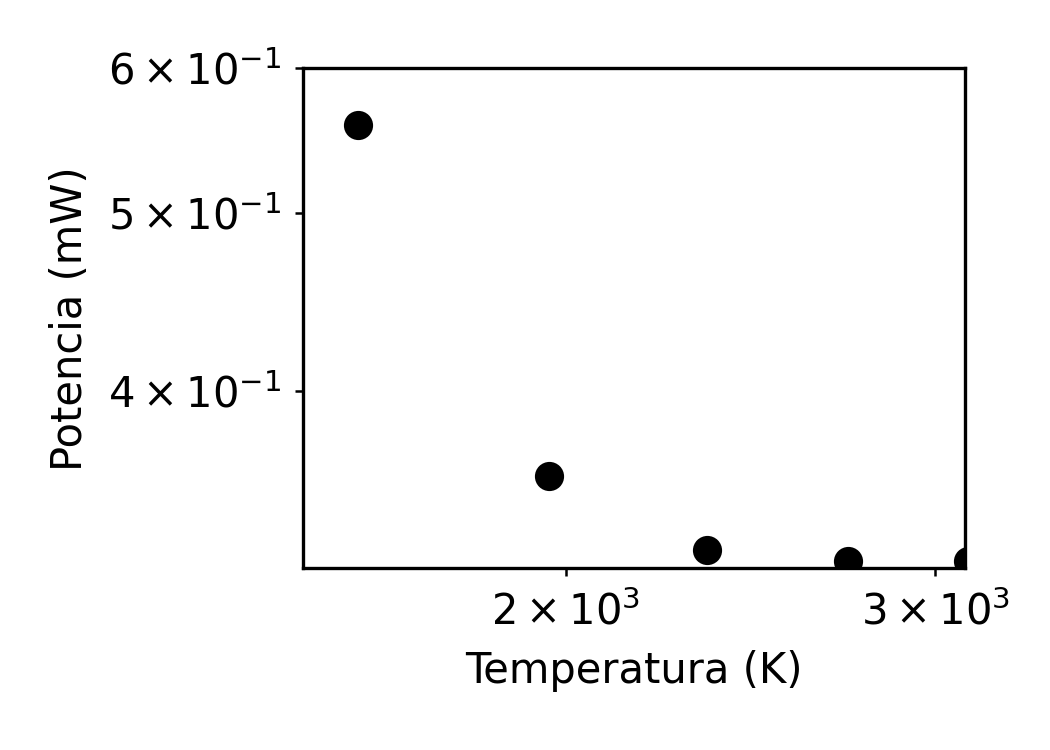
\includegraphics[scale=0.9]{resultados/imagenes/stefan.png}
	\end{center}
	\caption{Potencia radiada en función de la temperatura}
\end{figure}

\begin{figure}
	\begin{center}
		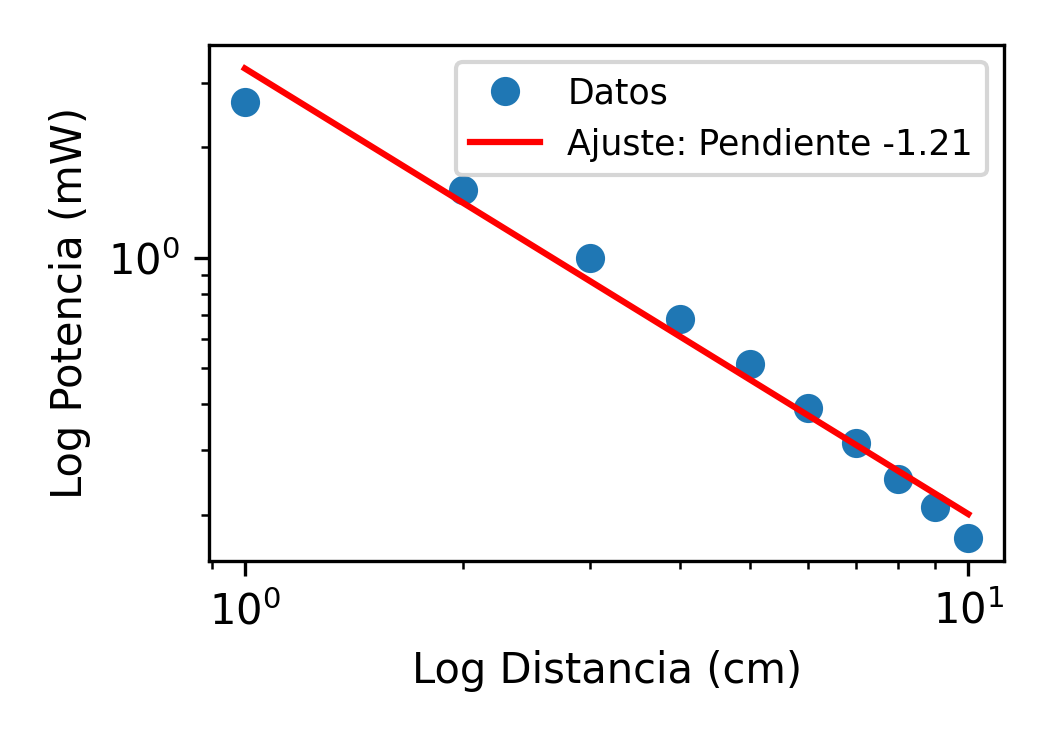
\includegraphics[scale=0.9]{resultados/imagenes/distancia.png}
	\end{center}
	\caption{Potencia en función de la distancia, a una temperatura constante. T = 2873K}
\end{figure}
